\steppingstone{What Happens When Everything Grows?}
\label{stone:growing}

Until now nothing has changed except the number of pieces.

Addition combined two collections.

Subtraction removed one collection from another.

The pieces themselves never changed.

Growth is different.

Suppose every short edge grows until it becomes exactly one long edge.

That is easy to picture.

Now ask the same question about a long edge.

What does it become?

Do not guess.

Look at Figure~\ref{fig:growing}.

\begin{figure}[htbp]
\centering
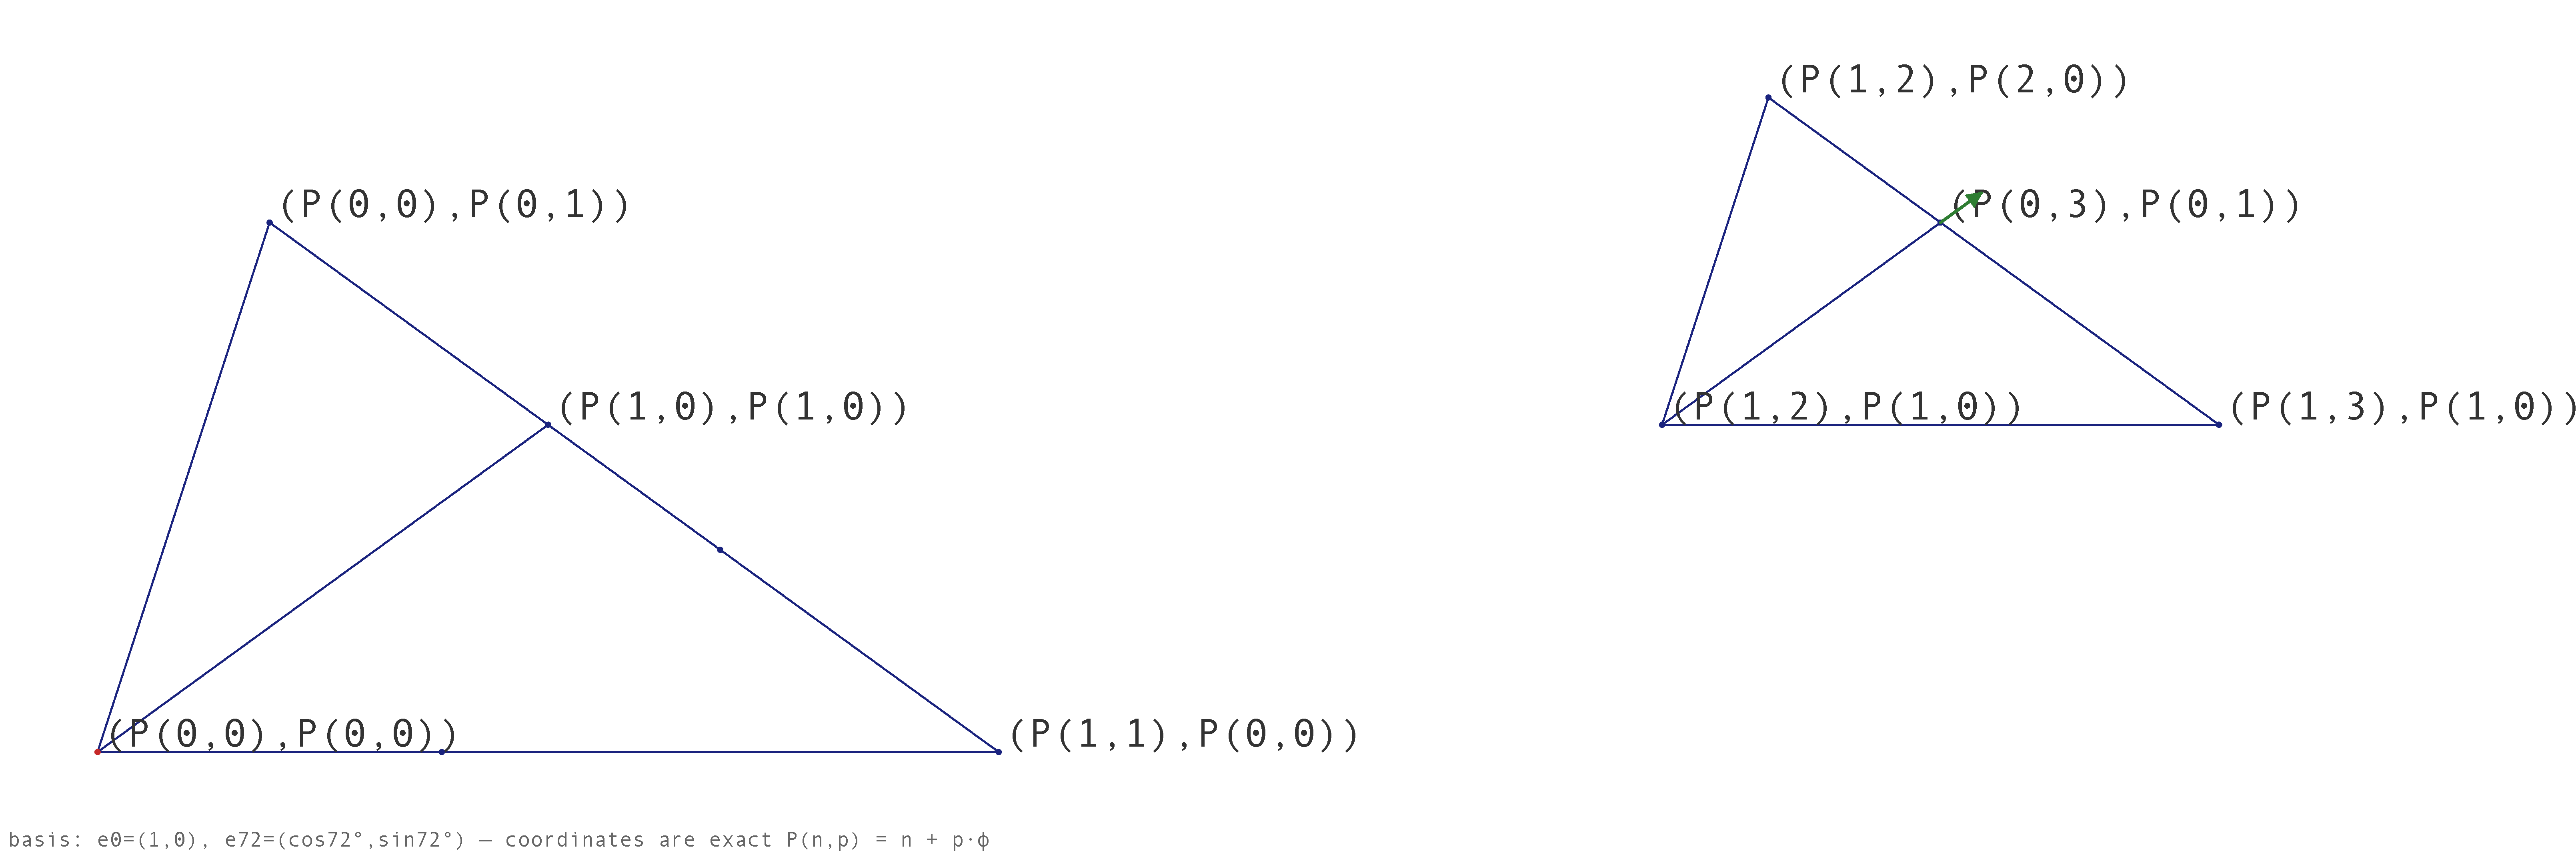
\includegraphics[width=.92\textwidth]{figures/turtle/growing.pdf}
\caption{Growing a golden triangle. The enlarged construction is built from the same two edge lengths.}
\label{fig:growing}
\end{figure}

The picture answers both questions.

A short edge becomes one long edge.

A long edge becomes one short edge and one long edge.

Nothing else appears.

No third length is created.

The same two pieces simply rearrange themselves.

The familiar identity

\[
\varphi^{2}=\varphi+1
\]

is nothing more than a compact description of that picture.

The geometry came first.

The equation came afterward.

\section*{Growing One Collection}

Suppose a collection contains

\[
P(3,2).
\]

The three short pieces each become one long piece.

The two long pieces each become one short piece and one long piece.

The result is easily counted.

\begin{center}
\begin{tabular}{rcl}
Before & $\longrightarrow$ & After \\
\hline
3 short & & 3 long \\
2 long  & & 2 short + 2 long \\
\hline
         & & 2 short + 5 long
\end{tabular}
\end{center}

The grown collection is therefore

\[
P(2,5).
\]

Nothing has been multiplied.

Nothing has been approximated.

We simply counted what the geometry produced.

Exactly the same reasoning works for every PhiBase collection:

\[
P(n,p)\longrightarrow P(p,n+p).
\]

The rule is only a summary.

The construction is the real mathematics.

\section*{Following the Growth}

Beginning with one short unit,

\[
P(1,0),
\]

the first few growth steps are

\begin{center}
\begin{tabular}{cl}
Before & After \\
\hline
$P(1,0)$ & $P(0,1)$ \\
$P(0,1)$ & $P(1,1)$ \\
$P(1,1)$ & $P(1,2)$ \\
$P(1,2)$ & $P(2,3)$ \\
$P(2,3)$ & $P(3,5)$
\end{tabular}
\end{center}

Every row is produced by exactly the same construction.

The arithmetic merely keeps count.

\section*{Builder's Notebook}

Continue the table six more rows.

Do not use decimal numbers.

Do not multiply.

Simply let every short edge become one long edge, and every long edge become one short edge and one long edge.

The geometry will produce the arithmetic for you.

\section*{Looking Ahead}

Growing by \(\varphi\) turned out to be surprisingly gentle.

Was that simply good fortune?

Or can every PhiBase multiplication be understood in the same way?
